\section{Mô hình Model-View-Controller}
Mô hình Model-View-Controller viết tắt là MVC, là một mô hình được sử dụng rộng rãi trong các dự án phát triển phần mềm hệ thống web. Mô hình được tạo nên từ ba thành phần, mỗi thành phần tương ứng với một chức năng trong mô hình.
\begin{itemize}
    \item Model là bộ phận có nhiệm vụ lưu trữ toàn bộ dữ liệu của ứng dụng. Model chứa tất cả các hàm, phương thức truy vấn trực tiếp với dữ liệu. Bộ phận này là cầu nối giữa hai thành phần Controller và View ở bên dưới. 
    \item View là thành phần giao diện người dùng, thành phần này có nhiệm vụ gửi yêu cầu đến Controller để lấy dữ liệu và hiển thị nội dung lên giao diện.
    \item Controller có nhiệm vụ tiếp nhận yêu cầu từ phía người dùng thông qua View và lấy dữ liệu tương ứng từ Model để trả về cho người dùng
\end{itemize}
\begin{center}
  \captionsetup{type=figure}
  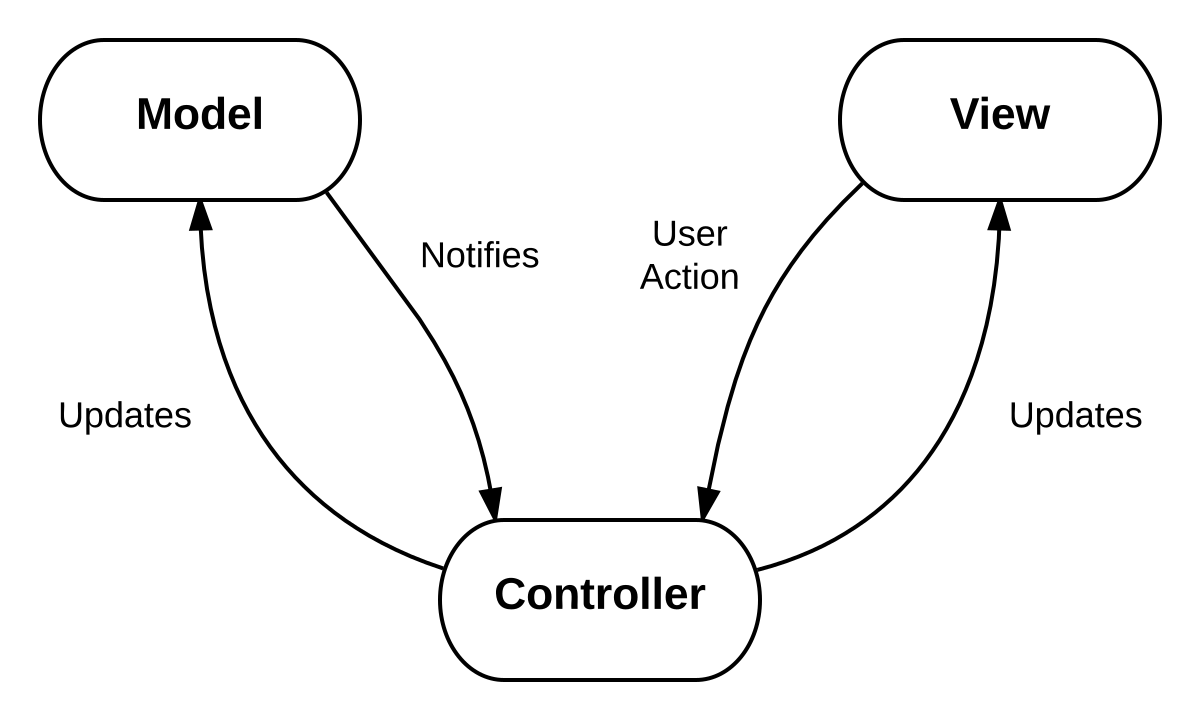
\includegraphics[width=10cm]{img/MVC.png}
  \captionof{figure}{Mô hình MVC}
\end{center}
\indent Hệ thống được chia ra các thành phần riêng biệt với nhau nên trong quá trình kiểm thử sẽ dễ dàng phát hiện và chỉnh sửa lỗi. Bên cạnh đó, việc nâng cấp phần mềm cũng trở nên dễ dàng hơn
